\documentclass[12pt]{article}

\usepackage{hyperref}
\usepackage{graphicx}
\usepackage{booktabs}
\usepackage{geometry}
\usepackage{tabularx}
\usepackage{float}
\usepackage[none]{hyphenat}
\usepackage{setspace}
\usepackage{subcaption}
\usepackage{titlesec}
\usepackage{amsmath}

\geometry{margin=1in}
\setstretch{0.96}

\titlespacing*{\section}{0pt}{10pt}{4pt}

\setlength{\parindent}{0pt}
\setlength{\parskip}{6pt}

\title{Labwork 3}
\author{Trinh Thanh Vinh - 2540110}
\date{\today}

\begin{document}

\maketitle

\section{Introduction}
In this labwork, we implement the logistic regression algorithm using gradient descent to find the best-fitting line for a given dataset. We will analyze the convergence of the algorithm and observe how different learning rates affect the results.
\section{Implementation and Experimentation}
The dataset used in this labwork is \texttt{loan2.csv}, which consists of samples with two input features --- \textbf{Experience} ($x^{(1)}$) and \textbf{Salary} ($x^{(2)}$) --- and a binary target label $y \in \{0, 1\}$ indicating whether a loan was approved. The goal of logistic regression is to find the parameters $w_1$, $w_2$, and $w_0$ such that the model
\[
\hat{y} = \sigma(w_1 x^{(1)} + w_2 x^{(2)} + w_0)
\]
best separates the two classes, where $\sigma$ is the sigmoid function defined as
\[
\sigma(z) = \frac{1}{1 + e^{-z}}.
\]
This means we want to find $(w_1, w_2, w_0)$ that minimizes the loss function:
\[
J = -\frac{1}{N} \sum_{i=1}^{N} \left( y_i(w_1 x_i^{(1)} + w_2 x_i^{(2)} + w_0) - \log\left(1 + e^{w_1 x_i^{(1)} + w_2 x_i^{(2)} + w_0}\right) \right)
\]
where $N$ is the number of data points.

All the related functions and the gradient descent algorithm are implemented in the Python file \texttt{labwork2\_logistic.ipynb}. The main components of the implementation include:
\begin{itemize}
    \item The loss function $J(w_1, w_2, w_0)$ which we want to minimize, defined as:
    \[
    J = -\frac{1}{N} \sum_{i=1}^{N} \left( y_i(w_1 x_i^{(1)} + w_2 x_i^{(2)} + w_0) - \log\left(1 + e^{w_1 x_i^{(1)} + w_2 x_i^{(2)} + w_0}\right) \right)
    \]
    \item The derivatives of the loss function with respect to $w_1$, $w_2$, and $w_0$, computed using the formulas:
    \[
    \frac{\partial J}{\partial w_0} = \frac{1}{N} \sum_{i=1}^{N} \left( -y_i + \left(1 - \sigma(-(w_1 x_i^{(1)} + w_2 x_i^{(2)} + w_0))\right) \right)
    \]
    \[
    \frac{\partial J}{\partial w_1} = \frac{1}{N} \sum_{i=1}^{N} \left( -y_i x_i^{(1)} + x_i^{(1)}\left(1 - \sigma(-(w_1 x_i^{(1)} + w_2 x_i^{(2)} + w_0))\right) \right)
    \]
    \[
    \frac{\partial J}{\partial w_2} = \frac{1}{N} \sum_{i=1}^{N} \left( -y_i x_i^{(2)} + x_i^{(2)}\left(1 - \sigma(-(w_1 x_i^{(1)} + w_2 x_i^{(2)} + w_0))\right) \right)
    \]
    \item The gradient descent algorithm that updates the values of $w_1$, $w_2$, and $w_0$ at each iteration based on the computed gradients and a specified learning rate $\ell$:
    \[
    w_k \leftarrow w_k - \ell \cdot \frac{\partial J}{\partial w_k}, \quad k \in \{0, 1, 2\}
    \]
    The update stops when the change in the loss function between two consecutive iterations is less than a specified threshold $\varepsilon = 10^{-6}$, indicating that the algorithm has converged to a minimum.
\end{itemize}

\section{Results and Discussion}
With this problem, we set the initial values of \( w_1 \), \(w_2 \), and \( w_0 \) to 1, 0, and 0 respectively. The initial learning rate is set at 0.001. The algorithm converge after over 96000 steps, with the final results being \( w_1 \approx 2.16 \), \( w_2 \approx 0.14 \), and \( w_0 \approx -3.15 \). The fitted regression line is plotted in the figure below, showing how the model separates the data points based on the learned parameters.
\begin{figure}[h]
    \centering
    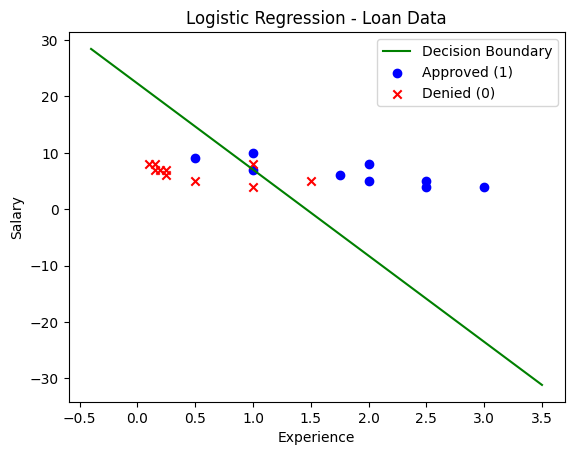
\includegraphics[width=0.5\textwidth]{figurelab31.png}
    \caption{Data points and the fitted regression line}
\end{figure}

With a lower learning rate of 0.0001, unlike the previous two labworks, the algorithm converges much faster after only 7107 steps, with the final parameters being \( w_1 \approx 0.92 \), \( w_2 \approx -0.25 \), and \( w_0 \approx 0.79 \). The fitted regression line is plotted in the figure below, showing a different separation of the data points compared to the previous case, which shows that the choice of learning rate can significantly affect the convergence and the final model parameters.
\begin{figure}[h]
    \centering
    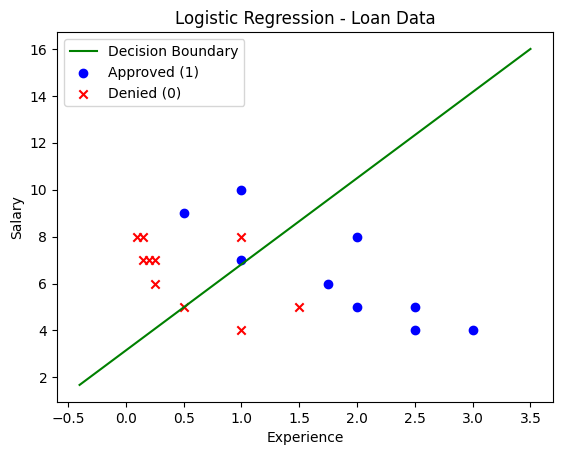
\includegraphics[width=0.5\textwidth]{figurelab32.png}
    \caption{Data points and the fitted regression line with a lower learning rate}
\end{figure}

Finally, with a higher learning rate of 0.1, the algorithm converges after over 13000 steps, with the final parameters being \( w_1 \approx 4.54 \), \( w_2 \approx 1.27 \), and \( w_0 \approx -13.57 \). The fitted regression line is plotted in the figure below, showing the model's performance with the higher learning rate.
\begin{figure}[h]
    \centering
    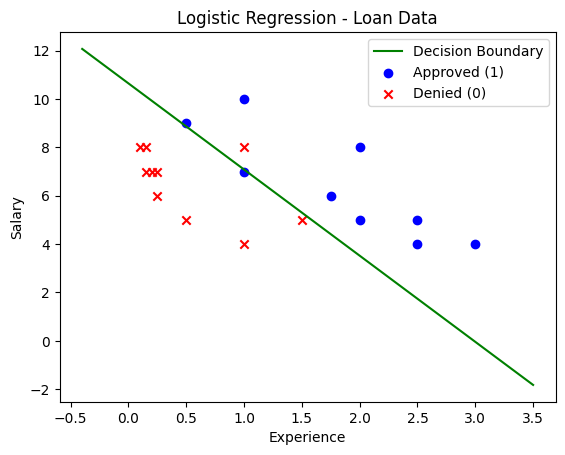
\includegraphics[width=0.5\textwidth]{figurelab33.png}
    \caption{Data points and the fitted regression line with a higher learning rate}
\end{figure}

\end{document}